
% Default to the notebook output style

    


% Inherit from the specified cell style.




    
\documentclass[11pt]{article}

    
    
    \usepackage[T1]{fontenc}
    % Nicer default font (+ math font) than Computer Modern for most use cases
    \usepackage{mathpazo}

    % Basic figure setup, for now with no caption control since it's done
    % automatically by Pandoc (which extracts ![](path) syntax from Markdown).
    \usepackage{graphicx}
    % We will generate all images so they have a width \maxwidth. This means
    % that they will get their normal width if they fit onto the page, but
    % are scaled down if they would overflow the margins.
    \makeatletter
    \def\maxwidth{\ifdim\Gin@nat@width>\linewidth\linewidth
    \else\Gin@nat@width\fi}
    \makeatother
    \let\Oldincludegraphics\includegraphics
    % Set max figure width to be 80% of text width, for now hardcoded.
    \renewcommand{\includegraphics}[1]{\Oldincludegraphics[width=.8\maxwidth]{#1}}
    % Ensure that by default, figures have no caption (until we provide a
    % proper Figure object with a Caption API and a way to capture that
    % in the conversion process - todo).
    \usepackage{caption}
    \DeclareCaptionLabelFormat{nolabel}{}
    \captionsetup{labelformat=nolabel}

    \usepackage{adjustbox} % Used to constrain images to a maximum size 
    \usepackage{xcolor} % Allow colors to be defined
    \usepackage{enumerate} % Needed for markdown enumerations to work
    \usepackage{geometry} % Used to adjust the document margins
    \usepackage{amsmath} % Equations
    \usepackage{amssymb} % Equations
    \usepackage{textcomp} % defines textquotesingle
    % Hack from http://tex.stackexchange.com/a/47451/13684:
    \AtBeginDocument{%
        \def\PYZsq{\textquotesingle}% Upright quotes in Pygmentized code
    }
    \usepackage{upquote} % Upright quotes for verbatim code
    \usepackage{eurosym} % defines \euro
    \usepackage[mathletters]{ucs} % Extended unicode (utf-8) support
    \usepackage[utf8x]{inputenc} % Allow utf-8 characters in the tex document
    \usepackage{fancyvrb} % verbatim replacement that allows latex
    \usepackage{grffile} % extends the file name processing of package graphics 
                         % to support a larger range 
    % The hyperref package gives us a pdf with properly built
    % internal navigation ('pdf bookmarks' for the table of contents,
    % internal cross-reference links, web links for URLs, etc.)
    \usepackage{hyperref}
    \usepackage{longtable} % longtable support required by pandoc >1.10
    \usepackage{booktabs}  % table support for pandoc > 1.12.2
    \usepackage[inline]{enumitem} % IRkernel/repr support (it uses the enumerate* environment)
    \usepackage[normalem]{ulem} % ulem is needed to support strikethroughs (\sout)
                                % normalem makes italics be italics, not underlines
    

    
    
    % Colors for the hyperref package
    \definecolor{urlcolor}{rgb}{0,.145,.698}
    \definecolor{linkcolor}{rgb}{.71,0.21,0.01}
    \definecolor{citecolor}{rgb}{.12,.54,.11}

    % ANSI colors
    \definecolor{ansi-black}{HTML}{3E424D}
    \definecolor{ansi-black-intense}{HTML}{282C36}
    \definecolor{ansi-red}{HTML}{E75C58}
    \definecolor{ansi-red-intense}{HTML}{B22B31}
    \definecolor{ansi-green}{HTML}{00A250}
    \definecolor{ansi-green-intense}{HTML}{007427}
    \definecolor{ansi-yellow}{HTML}{DDB62B}
    \definecolor{ansi-yellow-intense}{HTML}{B27D12}
    \definecolor{ansi-blue}{HTML}{208FFB}
    \definecolor{ansi-blue-intense}{HTML}{0065CA}
    \definecolor{ansi-magenta}{HTML}{D160C4}
    \definecolor{ansi-magenta-intense}{HTML}{A03196}
    \definecolor{ansi-cyan}{HTML}{60C6C8}
    \definecolor{ansi-cyan-intense}{HTML}{258F8F}
    \definecolor{ansi-white}{HTML}{C5C1B4}
    \definecolor{ansi-white-intense}{HTML}{A1A6B2}

    % commands and environments needed by pandoc snippets
    % extracted from the output of `pandoc -s`
    \providecommand{\tightlist}{%
      \setlength{\itemsep}{0pt}\setlength{\parskip}{0pt}}
    \DefineVerbatimEnvironment{Highlighting}{Verbatim}{commandchars=\\\{\}}
    % Add ',fontsize=\small' for more characters per line
    \newenvironment{Shaded}{}{}
    \newcommand{\KeywordTok}[1]{\textcolor[rgb]{0.00,0.44,0.13}{\textbf{{#1}}}}
    \newcommand{\DataTypeTok}[1]{\textcolor[rgb]{0.56,0.13,0.00}{{#1}}}
    \newcommand{\DecValTok}[1]{\textcolor[rgb]{0.25,0.63,0.44}{{#1}}}
    \newcommand{\BaseNTok}[1]{\textcolor[rgb]{0.25,0.63,0.44}{{#1}}}
    \newcommand{\FloatTok}[1]{\textcolor[rgb]{0.25,0.63,0.44}{{#1}}}
    \newcommand{\CharTok}[1]{\textcolor[rgb]{0.25,0.44,0.63}{{#1}}}
    \newcommand{\StringTok}[1]{\textcolor[rgb]{0.25,0.44,0.63}{{#1}}}
    \newcommand{\CommentTok}[1]{\textcolor[rgb]{0.38,0.63,0.69}{\textit{{#1}}}}
    \newcommand{\OtherTok}[1]{\textcolor[rgb]{0.00,0.44,0.13}{{#1}}}
    \newcommand{\AlertTok}[1]{\textcolor[rgb]{1.00,0.00,0.00}{\textbf{{#1}}}}
    \newcommand{\FunctionTok}[1]{\textcolor[rgb]{0.02,0.16,0.49}{{#1}}}
    \newcommand{\RegionMarkerTok}[1]{{#1}}
    \newcommand{\ErrorTok}[1]{\textcolor[rgb]{1.00,0.00,0.00}{\textbf{{#1}}}}
    \newcommand{\NormalTok}[1]{{#1}}
    
    % Additional commands for more recent versions of Pandoc
    \newcommand{\ConstantTok}[1]{\textcolor[rgb]{0.53,0.00,0.00}{{#1}}}
    \newcommand{\SpecialCharTok}[1]{\textcolor[rgb]{0.25,0.44,0.63}{{#1}}}
    \newcommand{\VerbatimStringTok}[1]{\textcolor[rgb]{0.25,0.44,0.63}{{#1}}}
    \newcommand{\SpecialStringTok}[1]{\textcolor[rgb]{0.73,0.40,0.53}{{#1}}}
    \newcommand{\ImportTok}[1]{{#1}}
    \newcommand{\DocumentationTok}[1]{\textcolor[rgb]{0.73,0.13,0.13}{\textit{{#1}}}}
    \newcommand{\AnnotationTok}[1]{\textcolor[rgb]{0.38,0.63,0.69}{\textbf{\textit{{#1}}}}}
    \newcommand{\CommentVarTok}[1]{\textcolor[rgb]{0.38,0.63,0.69}{\textbf{\textit{{#1}}}}}
    \newcommand{\VariableTok}[1]{\textcolor[rgb]{0.10,0.09,0.49}{{#1}}}
    \newcommand{\ControlFlowTok}[1]{\textcolor[rgb]{0.00,0.44,0.13}{\textbf{{#1}}}}
    \newcommand{\OperatorTok}[1]{\textcolor[rgb]{0.40,0.40,0.40}{{#1}}}
    \newcommand{\BuiltInTok}[1]{{#1}}
    \newcommand{\ExtensionTok}[1]{{#1}}
    \newcommand{\PreprocessorTok}[1]{\textcolor[rgb]{0.74,0.48,0.00}{{#1}}}
    \newcommand{\AttributeTok}[1]{\textcolor[rgb]{0.49,0.56,0.16}{{#1}}}
    \newcommand{\InformationTok}[1]{\textcolor[rgb]{0.38,0.63,0.69}{\textbf{\textit{{#1}}}}}
    \newcommand{\WarningTok}[1]{\textcolor[rgb]{0.38,0.63,0.69}{\textbf{\textit{{#1}}}}}
    
    
    % Define a nice break command that doesn't care if a line doesn't already
    % exist.
    \def\br{\hspace*{\fill} \\* }
    % Math Jax compatability definitions
    \def\gt{>}
    \def\lt{<}
    % Document parameters
    \title{Final\_Porject\_05-09-18}
    
    
    

    % Pygments definitions
    
\makeatletter
\def\PY@reset{\let\PY@it=\relax \let\PY@bf=\relax%
    \let\PY@ul=\relax \let\PY@tc=\relax%
    \let\PY@bc=\relax \let\PY@ff=\relax}
\def\PY@tok#1{\csname PY@tok@#1\endcsname}
\def\PY@toks#1+{\ifx\relax#1\empty\else%
    \PY@tok{#1}\expandafter\PY@toks\fi}
\def\PY@do#1{\PY@bc{\PY@tc{\PY@ul{%
    \PY@it{\PY@bf{\PY@ff{#1}}}}}}}
\def\PY#1#2{\PY@reset\PY@toks#1+\relax+\PY@do{#2}}

\expandafter\def\csname PY@tok@w\endcsname{\def\PY@tc##1{\textcolor[rgb]{0.73,0.73,0.73}{##1}}}
\expandafter\def\csname PY@tok@c\endcsname{\let\PY@it=\textit\def\PY@tc##1{\textcolor[rgb]{0.25,0.50,0.50}{##1}}}
\expandafter\def\csname PY@tok@cp\endcsname{\def\PY@tc##1{\textcolor[rgb]{0.74,0.48,0.00}{##1}}}
\expandafter\def\csname PY@tok@k\endcsname{\let\PY@bf=\textbf\def\PY@tc##1{\textcolor[rgb]{0.00,0.50,0.00}{##1}}}
\expandafter\def\csname PY@tok@kp\endcsname{\def\PY@tc##1{\textcolor[rgb]{0.00,0.50,0.00}{##1}}}
\expandafter\def\csname PY@tok@kt\endcsname{\def\PY@tc##1{\textcolor[rgb]{0.69,0.00,0.25}{##1}}}
\expandafter\def\csname PY@tok@o\endcsname{\def\PY@tc##1{\textcolor[rgb]{0.40,0.40,0.40}{##1}}}
\expandafter\def\csname PY@tok@ow\endcsname{\let\PY@bf=\textbf\def\PY@tc##1{\textcolor[rgb]{0.67,0.13,1.00}{##1}}}
\expandafter\def\csname PY@tok@nb\endcsname{\def\PY@tc##1{\textcolor[rgb]{0.00,0.50,0.00}{##1}}}
\expandafter\def\csname PY@tok@nf\endcsname{\def\PY@tc##1{\textcolor[rgb]{0.00,0.00,1.00}{##1}}}
\expandafter\def\csname PY@tok@nc\endcsname{\let\PY@bf=\textbf\def\PY@tc##1{\textcolor[rgb]{0.00,0.00,1.00}{##1}}}
\expandafter\def\csname PY@tok@nn\endcsname{\let\PY@bf=\textbf\def\PY@tc##1{\textcolor[rgb]{0.00,0.00,1.00}{##1}}}
\expandafter\def\csname PY@tok@ne\endcsname{\let\PY@bf=\textbf\def\PY@tc##1{\textcolor[rgb]{0.82,0.25,0.23}{##1}}}
\expandafter\def\csname PY@tok@nv\endcsname{\def\PY@tc##1{\textcolor[rgb]{0.10,0.09,0.49}{##1}}}
\expandafter\def\csname PY@tok@no\endcsname{\def\PY@tc##1{\textcolor[rgb]{0.53,0.00,0.00}{##1}}}
\expandafter\def\csname PY@tok@nl\endcsname{\def\PY@tc##1{\textcolor[rgb]{0.63,0.63,0.00}{##1}}}
\expandafter\def\csname PY@tok@ni\endcsname{\let\PY@bf=\textbf\def\PY@tc##1{\textcolor[rgb]{0.60,0.60,0.60}{##1}}}
\expandafter\def\csname PY@tok@na\endcsname{\def\PY@tc##1{\textcolor[rgb]{0.49,0.56,0.16}{##1}}}
\expandafter\def\csname PY@tok@nt\endcsname{\let\PY@bf=\textbf\def\PY@tc##1{\textcolor[rgb]{0.00,0.50,0.00}{##1}}}
\expandafter\def\csname PY@tok@nd\endcsname{\def\PY@tc##1{\textcolor[rgb]{0.67,0.13,1.00}{##1}}}
\expandafter\def\csname PY@tok@s\endcsname{\def\PY@tc##1{\textcolor[rgb]{0.73,0.13,0.13}{##1}}}
\expandafter\def\csname PY@tok@sd\endcsname{\let\PY@it=\textit\def\PY@tc##1{\textcolor[rgb]{0.73,0.13,0.13}{##1}}}
\expandafter\def\csname PY@tok@si\endcsname{\let\PY@bf=\textbf\def\PY@tc##1{\textcolor[rgb]{0.73,0.40,0.53}{##1}}}
\expandafter\def\csname PY@tok@se\endcsname{\let\PY@bf=\textbf\def\PY@tc##1{\textcolor[rgb]{0.73,0.40,0.13}{##1}}}
\expandafter\def\csname PY@tok@sr\endcsname{\def\PY@tc##1{\textcolor[rgb]{0.73,0.40,0.53}{##1}}}
\expandafter\def\csname PY@tok@ss\endcsname{\def\PY@tc##1{\textcolor[rgb]{0.10,0.09,0.49}{##1}}}
\expandafter\def\csname PY@tok@sx\endcsname{\def\PY@tc##1{\textcolor[rgb]{0.00,0.50,0.00}{##1}}}
\expandafter\def\csname PY@tok@m\endcsname{\def\PY@tc##1{\textcolor[rgb]{0.40,0.40,0.40}{##1}}}
\expandafter\def\csname PY@tok@gh\endcsname{\let\PY@bf=\textbf\def\PY@tc##1{\textcolor[rgb]{0.00,0.00,0.50}{##1}}}
\expandafter\def\csname PY@tok@gu\endcsname{\let\PY@bf=\textbf\def\PY@tc##1{\textcolor[rgb]{0.50,0.00,0.50}{##1}}}
\expandafter\def\csname PY@tok@gd\endcsname{\def\PY@tc##1{\textcolor[rgb]{0.63,0.00,0.00}{##1}}}
\expandafter\def\csname PY@tok@gi\endcsname{\def\PY@tc##1{\textcolor[rgb]{0.00,0.63,0.00}{##1}}}
\expandafter\def\csname PY@tok@gr\endcsname{\def\PY@tc##1{\textcolor[rgb]{1.00,0.00,0.00}{##1}}}
\expandafter\def\csname PY@tok@ge\endcsname{\let\PY@it=\textit}
\expandafter\def\csname PY@tok@gs\endcsname{\let\PY@bf=\textbf}
\expandafter\def\csname PY@tok@gp\endcsname{\let\PY@bf=\textbf\def\PY@tc##1{\textcolor[rgb]{0.00,0.00,0.50}{##1}}}
\expandafter\def\csname PY@tok@go\endcsname{\def\PY@tc##1{\textcolor[rgb]{0.53,0.53,0.53}{##1}}}
\expandafter\def\csname PY@tok@gt\endcsname{\def\PY@tc##1{\textcolor[rgb]{0.00,0.27,0.87}{##1}}}
\expandafter\def\csname PY@tok@err\endcsname{\def\PY@bc##1{\setlength{\fboxsep}{0pt}\fcolorbox[rgb]{1.00,0.00,0.00}{1,1,1}{\strut ##1}}}
\expandafter\def\csname PY@tok@kc\endcsname{\let\PY@bf=\textbf\def\PY@tc##1{\textcolor[rgb]{0.00,0.50,0.00}{##1}}}
\expandafter\def\csname PY@tok@kd\endcsname{\let\PY@bf=\textbf\def\PY@tc##1{\textcolor[rgb]{0.00,0.50,0.00}{##1}}}
\expandafter\def\csname PY@tok@kn\endcsname{\let\PY@bf=\textbf\def\PY@tc##1{\textcolor[rgb]{0.00,0.50,0.00}{##1}}}
\expandafter\def\csname PY@tok@kr\endcsname{\let\PY@bf=\textbf\def\PY@tc##1{\textcolor[rgb]{0.00,0.50,0.00}{##1}}}
\expandafter\def\csname PY@tok@bp\endcsname{\def\PY@tc##1{\textcolor[rgb]{0.00,0.50,0.00}{##1}}}
\expandafter\def\csname PY@tok@fm\endcsname{\def\PY@tc##1{\textcolor[rgb]{0.00,0.00,1.00}{##1}}}
\expandafter\def\csname PY@tok@vc\endcsname{\def\PY@tc##1{\textcolor[rgb]{0.10,0.09,0.49}{##1}}}
\expandafter\def\csname PY@tok@vg\endcsname{\def\PY@tc##1{\textcolor[rgb]{0.10,0.09,0.49}{##1}}}
\expandafter\def\csname PY@tok@vi\endcsname{\def\PY@tc##1{\textcolor[rgb]{0.10,0.09,0.49}{##1}}}
\expandafter\def\csname PY@tok@vm\endcsname{\def\PY@tc##1{\textcolor[rgb]{0.10,0.09,0.49}{##1}}}
\expandafter\def\csname PY@tok@sa\endcsname{\def\PY@tc##1{\textcolor[rgb]{0.73,0.13,0.13}{##1}}}
\expandafter\def\csname PY@tok@sb\endcsname{\def\PY@tc##1{\textcolor[rgb]{0.73,0.13,0.13}{##1}}}
\expandafter\def\csname PY@tok@sc\endcsname{\def\PY@tc##1{\textcolor[rgb]{0.73,0.13,0.13}{##1}}}
\expandafter\def\csname PY@tok@dl\endcsname{\def\PY@tc##1{\textcolor[rgb]{0.73,0.13,0.13}{##1}}}
\expandafter\def\csname PY@tok@s2\endcsname{\def\PY@tc##1{\textcolor[rgb]{0.73,0.13,0.13}{##1}}}
\expandafter\def\csname PY@tok@sh\endcsname{\def\PY@tc##1{\textcolor[rgb]{0.73,0.13,0.13}{##1}}}
\expandafter\def\csname PY@tok@s1\endcsname{\def\PY@tc##1{\textcolor[rgb]{0.73,0.13,0.13}{##1}}}
\expandafter\def\csname PY@tok@mb\endcsname{\def\PY@tc##1{\textcolor[rgb]{0.40,0.40,0.40}{##1}}}
\expandafter\def\csname PY@tok@mf\endcsname{\def\PY@tc##1{\textcolor[rgb]{0.40,0.40,0.40}{##1}}}
\expandafter\def\csname PY@tok@mh\endcsname{\def\PY@tc##1{\textcolor[rgb]{0.40,0.40,0.40}{##1}}}
\expandafter\def\csname PY@tok@mi\endcsname{\def\PY@tc##1{\textcolor[rgb]{0.40,0.40,0.40}{##1}}}
\expandafter\def\csname PY@tok@il\endcsname{\def\PY@tc##1{\textcolor[rgb]{0.40,0.40,0.40}{##1}}}
\expandafter\def\csname PY@tok@mo\endcsname{\def\PY@tc##1{\textcolor[rgb]{0.40,0.40,0.40}{##1}}}
\expandafter\def\csname PY@tok@ch\endcsname{\let\PY@it=\textit\def\PY@tc##1{\textcolor[rgb]{0.25,0.50,0.50}{##1}}}
\expandafter\def\csname PY@tok@cm\endcsname{\let\PY@it=\textit\def\PY@tc##1{\textcolor[rgb]{0.25,0.50,0.50}{##1}}}
\expandafter\def\csname PY@tok@cpf\endcsname{\let\PY@it=\textit\def\PY@tc##1{\textcolor[rgb]{0.25,0.50,0.50}{##1}}}
\expandafter\def\csname PY@tok@c1\endcsname{\let\PY@it=\textit\def\PY@tc##1{\textcolor[rgb]{0.25,0.50,0.50}{##1}}}
\expandafter\def\csname PY@tok@cs\endcsname{\let\PY@it=\textit\def\PY@tc##1{\textcolor[rgb]{0.25,0.50,0.50}{##1}}}

\def\PYZbs{\char`\\}
\def\PYZus{\char`\_}
\def\PYZob{\char`\{}
\def\PYZcb{\char`\}}
\def\PYZca{\char`\^}
\def\PYZam{\char`\&}
\def\PYZlt{\char`\<}
\def\PYZgt{\char`\>}
\def\PYZsh{\char`\#}
\def\PYZpc{\char`\%}
\def\PYZdl{\char`\$}
\def\PYZhy{\char`\-}
\def\PYZsq{\char`\'}
\def\PYZdq{\char`\"}
\def\PYZti{\char`\~}
% for compatibility with earlier versions
\def\PYZat{@}
\def\PYZlb{[}
\def\PYZrb{]}
\makeatother


    % Exact colors from NB
    \definecolor{incolor}{rgb}{0.0, 0.0, 0.5}
    \definecolor{outcolor}{rgb}{0.545, 0.0, 0.0}



    
    % Prevent overflowing lines due to hard-to-break entities
    \sloppy 
    % Setup hyperref package
    \hypersetup{
      breaklinks=true,  % so long urls are correctly broken across lines
      colorlinks=true,
      urlcolor=urlcolor,
      linkcolor=linkcolor,
      citecolor=citecolor,
      }
    % Slightly bigger margins than the latex defaults
    
    \geometry{verbose,tmargin=1in,bmargin=1in,lmargin=1in,rmargin=1in}
    
    

    \begin{document}
    
    
    \maketitle
    
    

    
    \#

Analyzing and Measuring Rising Sea Levels

\textbf{Authors: TingFang Pan and Wendy Carolina Velasquez Ebanks}

    \begin{Verbatim}[commandchars=\\\{\}]
{\color{incolor}In [{\color{incolor}1}]:} \PY{c+c1}{\PYZsh{}Libraries  required for the resalization of this project}
        \PY{k+kn}{import} \PY{n+nn}{nbconvert}
        \PY{k+kn}{import} \PY{n+nn}{pandas} \PY{k}{as} \PY{n+nn}{pd}
        \PY{k+kn}{import} \PY{n+nn}{numpy} \PY{k}{as} \PY{n+nn}{np}
        \PY{k+kn}{from} \PY{n+nn}{PIL} \PY{k}{import} \PY{n}{Image}
        \PY{o}{\PYZpc{}}\PY{k}{matplotlib} inline
        \PY{k+kn}{import} \PY{n+nn}{matplotlib}\PY{n+nn}{.}\PY{n+nn}{pyplot} \PY{k}{as} \PY{n+nn}{plt}
        \PY{k+kn}{from} \PY{n+nn}{mpl\PYZus{}toolkits}\PY{n+nn}{.}\PY{n+nn}{basemap} \PY{k}{import} \PY{n}{Basemap}
        \PY{k+kn}{import} \PY{n+nn}{os}
        \PY{k+kn}{import} \PY{n+nn}{IPython}
\end{Verbatim}


    \subsection{I. Introduction}\label{i.-introduction}

    In the last years, we have seen an accelerating rising on sea levels
around the world. As such, our intend with the realization of this
project is to analyze and measure sea levels in both coastsof the US, in
order to identify and predict how this will affect the main land. By
doing this we will be able to have a better perspective of the
vulnerable areas, that could suffer from the rising sea levels in
subsequent years based on the predictions calculated. The data used for
this study is collected from National Oceanic Atmospheric Administration
(NOAA)'s website on sea levels. We did the necessary processing for the
\textbf{US dataset only} and particulalry on three years (1997, 2008,
and 2016), and data from 2000 to 2016 for predictions and forecasting on
subsequent years. We will calculate the probability of danger and
vulnerability of certain areas based on the predictions previously
calcuated by using machine learning algorithms such as the Time Series
Model. The subject is worth discussing as it has a direct impact on
everyone as well as higher impact on future generations.

    \begin{Verbatim}[commandchars=\\\{\}]
{\color{incolor}In [{\color{incolor}7}]:} \PY{c+c1}{\PYZsh{} defines the size of the image displayed}
        \PY{n}{plt}\PY{o}{.}\PY{n}{figure}\PY{p}{(}\PY{n}{figsize}\PY{o}{=}\PY{p}{(}\PY{l+m+mi}{8}\PY{p}{,} \PY{l+m+mi}{8}\PY{p}{)}\PY{p}{)}
        
        \PY{c+c1}{\PYZsh{}Projection type}
        \PY{n}{worldMap} \PY{o}{=} \PY{n}{Basemap}\PY{p}{(}\PY{n}{projection}\PY{o}{=}\PY{l+s+s1}{\PYZsq{}}\PY{l+s+s1}{ortho}\PY{l+s+s1}{\PYZsq{}}\PY{p}{,} \PY{n}{resolution}\PY{o}{=}\PY{k+kc}{None}\PY{p}{,} \PY{n}{lat\PYZus{}0}\PY{o}{=}\PY{l+m+mi}{50}\PY{p}{,} \PY{n}{lon\PYZus{}0}\PY{o}{=}\PY{o}{\PYZhy{}}\PY{l+m+mi}{100}\PY{p}{)}
        
        \PY{c+c1}{\PYZsh{} defines the color of the map}
        \PY{n}{worldMap}\PY{o}{.}\PY{n}{bluemarble}\PY{p}{(}\PY{n}{scale}\PY{o}{=}\PY{l+m+mf}{0.5}\PY{p}{)}\PY{p}{;}
        \PY{n}{plt}\PY{o}{.}\PY{n}{title}\PY{p}{(}\PY{l+s+s2}{\PYZdq{}}\PY{l+s+s2}{The American and both oceans in the globe}\PY{l+s+s2}{\PYZdq{}}\PY{p}{)}
\end{Verbatim}


    \begin{Verbatim}[commandchars=\\\{\}]
C:\textbackslash{}Users\textbackslash{}Wendy\textbackslash{}Anaconda3\textbackslash{}lib\textbackslash{}site-packages\textbackslash{}mpl\_toolkits\textbackslash{}basemap\textbackslash{}\_\_init\_\_.py:1711: MatplotlibDeprecationWarning: The axesPatch function was deprecated in version 2.1. Use Axes.patch instead.
  if limb is not ax.axesPatch:

    \end{Verbatim}

\begin{Verbatim}[commandchars=\\\{\}]
{\color{outcolor}Out[{\color{outcolor}7}]:} Text(0.5,1,'The American and both oceans in the globe')
\end{Verbatim}
            
    \begin{center}
    \adjustimage{max size={0.9\linewidth}{0.9\paperheight}}{output_4_2.png}
    \end{center}
    { \hspace*{\fill} \\}
    
    \subsection{II. Background}\label{ii.-background}

Sea levels are measured around the world and through tide stations and
satellite laser altimeters. The tide stations around the globe tell the
story of what is happening at a local level by measuring the height of
the water along the coast and relative to a specific point on land
\href{https://oceanservice.noaa.gov/facts/sealevel.html}{{[}3{]}}.

As such research and records on sea level discuss the increasing
acceleration on sea levels for the last 40 years. On "\emph{A 20th
century acceleration in global sea-level rise}" paper from Church and
White (2006), they worked on data from time period 1950 to 2000, on
which they found a significanr acceleration on sea levels starting back
on1993 and subsequent years. They also made measurements on sea level
data dating on 1870 and found a significant sea‐level rise from January
1870 to December 2004 of 195 mm. An increasing rate of sea‐level rise of
1.7 ± 0.3 mm yr−1 up to that point in time and a significant
acceleration of sea‐level rise of 0.013 ± 0.006 mm yr−2
\href{https://agupubs.onlinelibrary.wiley.com/doi/full/10.1029/2005GL024826}{{[}1{]}}.

A common method among several papers on Sea Level measurements use
analyze sea level data, either local (usually tide gauge data) or
regional/global averages, in order to determine when and where sea level
may or may not have accelerated during a specific period of time during
the last century. It is consistent among studies that the increase is
not constant and in order to identify significance there need to be long
periods of time
\href{https://www.researchgate.net/publication/265467321_Time_and_tide_analysis_of_sea_level_time_series}{{[}2{]}}.

However, the majority of the studies and the ones mentioned above are
based on a time series method, this is due to several reasons; the
approach is useful to make predictions based on the past, allow us the
control of the process producing the series and give us a better
understanding of the mechanism behind the series generated. It give us
an intuitive description of the outputs in the time series.

    \subsection{III. Process and
Methodology}\label{iii.-process-and-methodology}

The process for this study consists in the preprocessing and collection
of datasets for each city on the East and West coasts of the United
States, provided by the National Oceanic Atmospheric Administration
(NOAA).

he datasets contain data recorded on sea levels by day, month and year
per each of the cities close to the edge of the beach on both sides.
This datasets were classified as \textbf{East} and \textbf{West} and
then each city dataset cleaned to obtain only three points in time
(1997, 2008, 2016) and data from 2000 to 2016 for predictions and
forecasting on subsequent years. Lastly, concatenated in order to make
just 2 big datasets that could then be more useful to fit the data in
the Time Series Model for prediction and forecasting.

    \begin{Verbatim}[commandchars=\\\{\}]
{\color{incolor}In [{\color{incolor}8}]:} \PY{n}{east\PYZus{}dir} \PY{o}{=} \PY{l+s+s2}{\PYZdq{}}\PY{l+s+s2}{DATA/east\PYZus{}new}\PY{l+s+s2}{\PYZdq{}}
        \PY{n}{west\PYZus{}dir} \PY{o}{=} \PY{l+s+s2}{\PYZdq{}}\PY{l+s+s2}{DATA/west\PYZus{}new}\PY{l+s+s2}{\PYZdq{}}
        \PY{n}{east\PYZus{}dir\PYZus{}list} \PY{o}{=} \PY{n}{os}\PY{o}{.}\PY{n}{listdir}\PY{p}{(}\PY{n}{east\PYZus{}dir}\PY{p}{)}
        \PY{n}{west\PYZus{}dir\PYZus{}list} \PY{o}{=} \PY{n}{os}\PY{o}{.}\PY{n}{listdir}\PY{p}{(}\PY{n}{west\PYZus{}dir}\PY{p}{)}
        \PY{n}{east\PYZus{}d\PYZus{}dict} \PY{o}{=} \PY{p}{\PYZob{}}\PY{p}{\PYZcb{}} \PY{c+c1}{\PYZsh{} key is a file name(string type), item is a dataframe}
        \PY{n}{east\PYZus{}h\PYZus{}dict} \PY{o}{=} \PY{p}{\PYZob{}}\PY{p}{\PYZcb{}}
        \PY{n}{west\PYZus{}d\PYZus{}dict} \PY{o}{=} \PY{p}{\PYZob{}}\PY{p}{\PYZcb{}}
        \PY{n}{west\PYZus{}h\PYZus{}dict} \PY{o}{=} \PY{p}{\PYZob{}}\PY{p}{\PYZcb{}}
        \PY{k}{for} \PY{n}{east\PYZus{}fname} \PY{o+ow}{in} \PY{n}{east\PYZus{}dir\PYZus{}list}\PY{p}{:}
            \PY{n}{file\PYZus{}directory} \PY{o}{=} \PY{n}{east\PYZus{}dir} \PY{o}{+} \PY{l+s+s2}{\PYZdq{}}\PY{l+s+s2}{/}\PY{l+s+s2}{\PYZdq{}} \PY{o}{+} \PY{n}{east\PYZus{}fname} 
            \PY{c+c1}{\PYZsh{}read csv file to dataframe from file\PYZus{}directory}
            
            \PY{n}{k} \PY{o}{=} \PY{n}{east\PYZus{}fname}\PY{o}{.}\PY{n}{rfind}\PY{p}{(}\PY{l+s+s2}{\PYZdq{}}\PY{l+s+s2}{.}\PY{l+s+s2}{\PYZdq{}}\PY{p}{)}
            \PY{n}{d\PYZus{}or\PYZus{}h\PYZus{}index} \PY{o}{=} \PY{n}{k} \PY{o}{\PYZhy{}} \PY{l+m+mi}{1} \PY{c+c1}{\PYZsh{}determine whether the file is about d or about h}
            
            \PY{k}{if}\PY{p}{(}\PY{n}{east\PYZus{}fname}\PY{p}{[}\PY{n}{d\PYZus{}or\PYZus{}h\PYZus{}index}\PY{p}{]} \PY{o}{==} \PY{l+s+s1}{\PYZsq{}}\PY{l+s+s1}{d}\PY{l+s+s1}{\PYZsq{}}\PY{p}{)}\PY{p}{:}
                \PY{n}{df\PYZus{}file} \PY{o}{=} \PY{n}{pd}\PY{o}{.}\PY{n}{read\PYZus{}csv}\PY{p}{(}\PY{n}{file\PYZus{}directory}\PY{p}{,}\PY{n}{names} \PY{o}{=} \PY{p}{[}\PY{l+s+s2}{\PYZdq{}}\PY{l+s+s2}{year}\PY{l+s+s2}{\PYZdq{}}\PY{p}{,} \PY{l+s+s2}{\PYZdq{}}\PY{l+s+s2}{month}\PY{l+s+s2}{\PYZdq{}}\PY{p}{,} \PY{l+s+s2}{\PYZdq{}}\PY{l+s+s2}{day}\PY{l+s+s2}{\PYZdq{}}\PY{p}{,} \PY{l+s+s2}{\PYZdq{}}\PY{l+s+s2}{sea\PYZus{}level}\PY{l+s+s2}{\PYZdq{}}\PY{p}{]}\PY{p}{)}
                \PY{n}{df\PYZus{}file}\PY{p}{[}\PY{l+s+s2}{\PYZdq{}}\PY{l+s+s2}{date}\PY{l+s+s2}{\PYZdq{}}\PY{p}{]} \PY{o}{=} \PY{n}{pd}\PY{o}{.}\PY{n}{to\PYZus{}datetime}\PY{p}{(}\PY{n}{df\PYZus{}file}\PY{p}{[}\PY{p}{[}\PY{l+s+s1}{\PYZsq{}}\PY{l+s+s1}{day}\PY{l+s+s1}{\PYZsq{}}\PY{p}{,}\PY{l+s+s1}{\PYZsq{}}\PY{l+s+s1}{month}\PY{l+s+s1}{\PYZsq{}}\PY{p}{,}\PY{l+s+s1}{\PYZsq{}}\PY{l+s+s1}{year}\PY{l+s+s1}{\PYZsq{}}\PY{p}{]}\PY{p}{]}\PY{p}{)}
                \PY{n}{east\PYZus{}d\PYZus{}dict}\PY{p}{[}\PY{n}{east\PYZus{}fname}\PY{p}{]} \PY{o}{=} \PY{n}{df\PYZus{}file}
            \PY{k}{else}\PY{p}{:}
                \PY{n}{df\PYZus{}file} \PY{o}{=} \PY{n}{pd}\PY{o}{.}\PY{n}{read\PYZus{}csv}\PY{p}{(}\PY{n}{file\PYZus{}directory}\PY{p}{,}\PY{n}{names} \PY{o}{=} \PY{p}{[}\PY{l+s+s2}{\PYZdq{}}\PY{l+s+s2}{year}\PY{l+s+s2}{\PYZdq{}}\PY{p}{,} \PY{l+s+s2}{\PYZdq{}}\PY{l+s+s2}{month}\PY{l+s+s2}{\PYZdq{}}\PY{p}{,} \PY{l+s+s2}{\PYZdq{}}\PY{l+s+s2}{day}\PY{l+s+s2}{\PYZdq{}}\PY{p}{,}\PY{l+s+s2}{\PYZdq{}}\PY{l+s+s2}{hour}\PY{l+s+s2}{\PYZdq{}}\PY{p}{,}\PY{l+s+s2}{\PYZdq{}}\PY{l+s+s2}{sea\PYZus{}level}\PY{l+s+s2}{\PYZdq{}}\PY{p}{]}\PY{p}{)}
                \PY{n}{df\PYZus{}file}\PY{p}{[}\PY{l+s+s2}{\PYZdq{}}\PY{l+s+s2}{date}\PY{l+s+s2}{\PYZdq{}}\PY{p}{]} \PY{o}{=} \PY{n}{pd}\PY{o}{.}\PY{n}{to\PYZus{}datetime}\PY{p}{(}\PY{n}{df\PYZus{}file}\PY{p}{[}\PY{p}{[}\PY{l+s+s1}{\PYZsq{}}\PY{l+s+s1}{day}\PY{l+s+s1}{\PYZsq{}}\PY{p}{,}\PY{l+s+s1}{\PYZsq{}}\PY{l+s+s1}{month}\PY{l+s+s1}{\PYZsq{}}\PY{p}{,}\PY{l+s+s1}{\PYZsq{}}\PY{l+s+s1}{year}\PY{l+s+s1}{\PYZsq{}}\PY{p}{]}\PY{p}{]}\PY{p}{)}
                \PY{n}{east\PYZus{}h\PYZus{}dict}\PY{p}{[}\PY{n}{east\PYZus{}fname}\PY{p}{]} \PY{o}{=} \PY{n}{df\PYZus{}file}
        
        \PY{k}{for} \PY{n}{west\PYZus{}fname} \PY{o+ow}{in} \PY{n}{west\PYZus{}dir\PYZus{}list}\PY{p}{:}
            \PY{n}{file\PYZus{}directory} \PY{o}{=} \PY{n}{west\PYZus{}dir} \PY{o}{+} \PY{l+s+s2}{\PYZdq{}}\PY{l+s+s2}{/}\PY{l+s+s2}{\PYZdq{}} \PY{o}{+} \PY{n}{west\PYZus{}fname} 
            \PY{c+c1}{\PYZsh{}read csv file to dataframe from file\PYZus{}directory}
            
            \PY{n}{k} \PY{o}{=} \PY{n}{west\PYZus{}fname}\PY{o}{.}\PY{n}{rfind}\PY{p}{(}\PY{l+s+s2}{\PYZdq{}}\PY{l+s+s2}{.}\PY{l+s+s2}{\PYZdq{}}\PY{p}{)}
            \PY{n}{d\PYZus{}or\PYZus{}h\PYZus{}index} \PY{o}{=} \PY{n}{k} \PY{o}{\PYZhy{}} \PY{l+m+mi}{1} \PY{c+c1}{\PYZsh{}determine whether the file is about d or about h}
            
            \PY{k}{if}\PY{p}{(}\PY{n}{west\PYZus{}fname}\PY{p}{[}\PY{n}{d\PYZus{}or\PYZus{}h\PYZus{}index}\PY{p}{]} \PY{o}{==} \PY{l+s+s1}{\PYZsq{}}\PY{l+s+s1}{d}\PY{l+s+s1}{\PYZsq{}}\PY{p}{)}\PY{p}{:}
                \PY{n}{df\PYZus{}file} \PY{o}{=} \PY{n}{pd}\PY{o}{.}\PY{n}{read\PYZus{}csv}\PY{p}{(}\PY{n}{file\PYZus{}directory}\PY{p}{,}\PY{n}{names} \PY{o}{=} \PY{p}{[}\PY{l+s+s2}{\PYZdq{}}\PY{l+s+s2}{year}\PY{l+s+s2}{\PYZdq{}}\PY{p}{,} \PY{l+s+s2}{\PYZdq{}}\PY{l+s+s2}{month}\PY{l+s+s2}{\PYZdq{}}\PY{p}{,} \PY{l+s+s2}{\PYZdq{}}\PY{l+s+s2}{day}\PY{l+s+s2}{\PYZdq{}}\PY{p}{,} \PY{l+s+s2}{\PYZdq{}}\PY{l+s+s2}{sea\PYZus{}level}\PY{l+s+s2}{\PYZdq{}}\PY{p}{]}\PY{p}{)}
                \PY{n}{df\PYZus{}file}\PY{p}{[}\PY{l+s+s2}{\PYZdq{}}\PY{l+s+s2}{date}\PY{l+s+s2}{\PYZdq{}}\PY{p}{]} \PY{o}{=} \PY{n}{pd}\PY{o}{.}\PY{n}{to\PYZus{}datetime}\PY{p}{(}\PY{n}{df\PYZus{}file}\PY{p}{[}\PY{p}{[}\PY{l+s+s1}{\PYZsq{}}\PY{l+s+s1}{day}\PY{l+s+s1}{\PYZsq{}}\PY{p}{,}\PY{l+s+s1}{\PYZsq{}}\PY{l+s+s1}{month}\PY{l+s+s1}{\PYZsq{}}\PY{p}{,}\PY{l+s+s1}{\PYZsq{}}\PY{l+s+s1}{year}\PY{l+s+s1}{\PYZsq{}}\PY{p}{]}\PY{p}{]}\PY{p}{)}
                \PY{n}{west\PYZus{}d\PYZus{}dict}\PY{p}{[}\PY{n}{west\PYZus{}fname}\PY{p}{]} \PY{o}{=} \PY{n}{df\PYZus{}file}
            \PY{k}{else}\PY{p}{:}
                \PY{n}{df\PYZus{}file} \PY{o}{=} \PY{n}{pd}\PY{o}{.}\PY{n}{read\PYZus{}csv}\PY{p}{(}\PY{n}{file\PYZus{}directory}\PY{p}{,}\PY{n}{names} \PY{o}{=} \PY{p}{[}\PY{l+s+s2}{\PYZdq{}}\PY{l+s+s2}{year}\PY{l+s+s2}{\PYZdq{}}\PY{p}{,} \PY{l+s+s2}{\PYZdq{}}\PY{l+s+s2}{month}\PY{l+s+s2}{\PYZdq{}}\PY{p}{,} \PY{l+s+s2}{\PYZdq{}}\PY{l+s+s2}{day}\PY{l+s+s2}{\PYZdq{}}\PY{p}{,}\PY{l+s+s2}{\PYZdq{}}\PY{l+s+s2}{hour}\PY{l+s+s2}{\PYZdq{}}\PY{p}{,}\PY{l+s+s2}{\PYZdq{}}\PY{l+s+s2}{sea\PYZus{}level}\PY{l+s+s2}{\PYZdq{}}\PY{p}{]}\PY{p}{)}
                \PY{n}{df\PYZus{}file}\PY{p}{[}\PY{l+s+s2}{\PYZdq{}}\PY{l+s+s2}{date}\PY{l+s+s2}{\PYZdq{}}\PY{p}{]} \PY{o}{=} \PY{n}{pd}\PY{o}{.}\PY{n}{to\PYZus{}datetime}\PY{p}{(}\PY{n}{df\PYZus{}file}\PY{p}{[}\PY{p}{[}\PY{l+s+s1}{\PYZsq{}}\PY{l+s+s1}{hour}\PY{l+s+s1}{\PYZsq{}}\PY{p}{,}\PY{l+s+s1}{\PYZsq{}}\PY{l+s+s1}{day}\PY{l+s+s1}{\PYZsq{}}\PY{p}{,}\PY{l+s+s1}{\PYZsq{}}\PY{l+s+s1}{month}\PY{l+s+s1}{\PYZsq{}}\PY{p}{,}\PY{l+s+s1}{\PYZsq{}}\PY{l+s+s1}{year}\PY{l+s+s1}{\PYZsq{}}\PY{p}{]}\PY{p}{]}\PY{p}{)}
                \PY{n}{west\PYZus{}h\PYZus{}dict}\PY{p}{[}\PY{n}{west\PYZus{}fname}\PY{p}{]} \PY{o}{=} \PY{n}{df\PYZus{}file}
        \PY{c+c1}{\PYZsh{}print([key for key in west\PYZus{}h\PYZus{}dict])}
        \PY{n+nb}{print}\PY{p}{(}\PY{n}{west\PYZus{}h\PYZus{}dict}\PY{p}{[}\PY{l+s+s2}{\PYZdq{}}\PY{l+s+s2}{Cordova\PYZus{}h.csv}\PY{l+s+s2}{\PYZdq{}}\PY{p}{]}\PY{p}{)}
\end{Verbatim}


    \begin{Verbatim}[commandchars=\\\{\}]
       year  month  day  hour  sea\_level                date
0      1997      1    1     0       4730 1997-01-01 00:00:00
1      1997      1    1     1       5060 1997-01-01 01:00:00
2      1997      1    1     2       5118 1997-01-01 02:00:00
3      1997      1    1     3       4968 1997-01-01 03:00:00
4      1997      1    1     4       4673 1997-01-01 04:00:00
5      1997      1    1     5       4257 1997-01-01 05:00:00
6      1997      1    1     6       3715 1997-01-01 06:00:00
7      1997      1    1     7       3228 1997-01-01 07:00:00
8      1997      1    1     8       2899 1997-01-01 08:00:00
9      1997      1    1     9       2904 1997-01-01 09:00:00
10     1997      1    1    10       3219 1997-01-01 10:00:00
11     1997      1    1    11       3794 1997-01-01 11:00:00
12     1997      1    1    12       4454 1997-01-01 12:00:00
13     1997      1    1    13       5031 1997-01-01 13:00:00
14     1997      1    1    14       5357 1997-01-01 14:00:00
15     1997      1    1    15       5416 1997-01-01 15:00:00
16     1997      1    1    16       5295 1997-01-01 16:00:00
17     1997      1    1    17       5028 1997-01-01 17:00:00
18     1997      1    1    18       4614 1997-01-01 18:00:00
19     1997      1    1    19       4151 1997-01-01 19:00:00
20     1997      1    1    20       3685 1997-01-01 20:00:00
21     1997      1    1    21       3371 1997-01-01 21:00:00
22     1997      1    1    22       3369 1997-01-01 22:00:00
23     1997      1    1    23       3690 1997-01-01 23:00:00
24     1997      1    2     0       4122 1997-01-02 00:00:00
25     1997      1    2     1       4512 1997-01-02 01:00:00
26     1997      1    2     2       4741 1997-01-02 02:00:00
27     1997      1    2     3       4791 1997-01-02 03:00:00
28     1997      1    2     4       4678 1997-01-02 04:00:00
29     1997      1    2     5       4431 1997-01-02 05:00:00
{\ldots}     {\ldots}    {\ldots}  {\ldots}   {\ldots}        {\ldots}                 {\ldots}
26298  2016     12   30    18       3214 2016-12-30 18:00:00
26299  2016     12   30    19       3950 2016-12-30 19:00:00
26300  2016     12   30    20       4724 2016-12-30 20:00:00
26301  2016     12   30    21       5426 2016-12-30 21:00:00
26302  2016     12   30    22       5843 2016-12-30 22:00:00
26303  2016     12   30    23       5817 2016-12-30 23:00:00
26304  2016     12   31     0       5331 2016-12-31 00:00:00
26305  2016     12   31     1       4569 2016-12-31 01:00:00
26306  2016     12   31     2       3501 2016-12-31 02:00:00
26307  2016     12   31     3       2440 2016-12-31 03:00:00
26308  2016     12   31     4       1427 2016-12-31 04:00:00
26309  2016     12   31     5       1092 2016-12-31 05:00:00
26310  2016     12   31     6       1180 2016-12-31 06:00:00
26311  2016     12   31     7       1820 2016-12-31 07:00:00
26312  2016     12   31     8       2732 2016-12-31 08:00:00
26313  2016     12   31     9       3626 2016-12-31 09:00:00
26314  2016     12   31    10       4377 2016-12-31 10:00:00
26315  2016     12   31    11       4946 2016-12-31 11:00:00
26316  2016     12   31    12       5124 2016-12-31 12:00:00
26317  2016     12   31    13       4783 2016-12-31 13:00:00
26318  2016     12   31    14       4127 2016-12-31 14:00:00
26319  2016     12   31    15       3440 2016-12-31 15:00:00
26320  2016     12   31    16       2774 2016-12-31 16:00:00
26321  2016     12   31    17       2474 2016-12-31 17:00:00
26322  2016     12   31    18       2633 2016-12-31 18:00:00
26323  2016     12   31    19       3165 2016-12-31 19:00:00
26324  2016     12   31    20       3895 2016-12-31 20:00:00
26325  2016     12   31    21       4633 2016-12-31 21:00:00
26326  2016     12   31    22       5250 2016-12-31 22:00:00
26327  2016     12   31    23       5538 2016-12-31 23:00:00

[26328 rows x 6 columns]

    \end{Verbatim}

    \subsubsection{Methodology: Time Series
Model}\label{methodology-time-series-model}

By definition A \textbf{"Time Series"} analysis is the process of using
statistical techniques to model and explain a time-dependent series of
data points. Time series forecasting is the process of using a model to
generate predictions (forecasts) for future events based on known past
events
\href{https://wiki.pentaho.com/display/DATAMINING/Time+Series+Analysis+and+Forecasting+with+Weka\#TimeSeriesAnalysisandForecastingwithWeka-1Introduction}{{[}4{]}}.
Consequently, this model fits our data for this study perfectly.

\begin{quote}
\begin{figure}
\centering
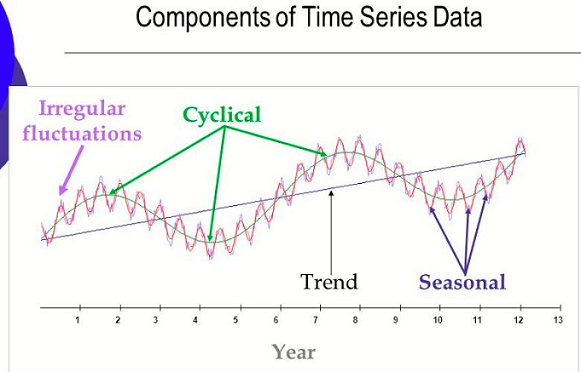
\includegraphics{timeseriesim.jpg}
\caption{time\_series\_graph}
\end{figure}
\end{quote}

Where we have observations \(X_1\ldots,X_n\) and \(X_t\) denotes the
observation at time 𝑡. In terms of machine learning, we consider the
prediction problem as a problem of supervised learning problem, where we
have to infer from historical data the possibly nonlinear dependance
between the input (past data sea levels) and the output (future of
rising sea levels). We will use methods to reduce trends, seasonality,
leaving the stationary to make the forecasts by using the following
equations to make the respective calculations that will provide the
desired results.

\begin{quote}
\subsubsection{The Autoregressive Model:
AR}\label{the-autoregressive-model-ar}

An autoregressive model predicts the response \(X_t\) using a linear
combination of past values of the variable. Parameterized by 𝑝, (the
number of past values to include).
\end{quote}

\begin{quote}
\[X_t = \mathbf\theta_0 + \mathbf\theta_1 X_(t-1) + \mathbf\theta_2 X_(t-2) + \mathbf\theta_p X_(t-p)\]
\end{quote}

\begin{quote}
\subsubsection{The ARIMA Model for Predictions and
Forecasting}\label{the-arima-model-for-predictions-and-forecasting}
\end{quote}

We Combined a autoregressive (AR) with the moving average (MA) model, to
get the ARIMA model.

𝑋′\& = 𝜃; + 𝜃"𝑋\&+" + 𝜃=𝑋\&+= + \ldots{}+
𝜃\textgreater{}𝑋\&+\textgreater{} + 𝛽; + 𝛽"𝜖\&+" + 𝛽=𝜖\&+= + \ldots{}+
𝛽A𝜖\&+A Note that now we are regressing on 𝑋′\&, which is the
differenced series 𝑋\&. The order of difference is determined by the the
parameter 𝑑. For example, if 𝑑 = 1: 𝑋′\& = X6 − X6+" for t = 2,
3,\ldots{},N So the ARIMA model is parameterized by: p (order of the AR
part), q (order of the MA part), and d (degree of differencing).

    \subsection{IV. Calculations, and
Results}\label{iv.-calculations-and-results}

    \begin{Verbatim}[commandchars=\\\{\}]
{\color{incolor}In [{\color{incolor} }]:} \PY{c+c1}{\PYZsh{}calculations}
\end{Verbatim}


    \begin{Verbatim}[commandchars=\\\{\}]
{\color{incolor}In [{\color{incolor}13}]:} \PY{c+c1}{\PYZsh{}dimensions of the figure}
         \PY{n}{fig} \PY{o}{=} \PY{n}{plt}\PY{o}{.}\PY{n}{figure}\PY{p}{(}\PY{n}{figsize}\PY{o}{=}\PY{p}{(}\PY{l+m+mi}{8}\PY{p}{,} \PY{l+m+mi}{8}\PY{p}{)}\PY{p}{)}
         
         \PY{c+c1}{\PYZsh{}Projection of the map}
         \PY{n}{USmap} \PY{o}{=} \PY{n}{Basemap}\PY{p}{(}\PY{n}{projection}\PY{o}{=}\PY{l+s+s1}{\PYZsq{}}\PY{l+s+s1}{lcc}\PY{l+s+s1}{\PYZsq{}}\PY{p}{,} \PY{n}{resolution}\PY{o}{=}\PY{k+kc}{None}\PY{p}{,} \PY{n}{width}\PY{o}{=}\PY{l+m+mf}{8E6}\PY{p}{,} \PY{n}{height}\PY{o}{=}\PY{l+m+mf}{8E6}\PY{p}{,} \PY{n}{lat\PYZus{}0}\PY{o}{=}\PY{l+m+mi}{45}\PY{p}{,} \PY{n}{lon\PYZus{}0}\PY{o}{=}\PY{o}{\PYZhy{}}\PY{l+m+mi}{100}\PY{p}{,}\PY{p}{)}
         
         \PY{c+c1}{\PYZsh{} Topografic Scale}
         \PY{n}{USmap}\PY{o}{.}\PY{n}{etopo}\PY{p}{(}\PY{n}{scale}\PY{o}{=}\PY{l+m+mf}{0.5}\PY{p}{,} \PY{n}{alpha}\PY{o}{=}\PY{l+m+mf}{0.5}\PY{p}{)}
         
         \PY{c+c1}{\PYZsh{} Map (long, lat) to (x, y) for plotting}
         \PY{c+c1}{\PYZsh{}coordinates of the points that signalize both coasts}
         \PY{n}{x}\PY{p}{,} \PY{n}{y} \PY{o}{=} \PY{n}{USmap}\PY{p}{(}\PY{o}{\PYZhy{}}\PY{l+m+mf}{121.5}\PY{p}{,} \PY{l+m+mf}{60.5}\PY{p}{)}
         \PY{n}{x1}\PY{p}{,} \PY{n}{y1} \PY{o}{=} \PY{n}{USmap}\PY{p}{(}\PY{o}{\PYZhy{}}\PY{l+m+mf}{127.3}\PY{p}{,} \PY{l+m+mf}{38.7}\PY{p}{)}
         
         \PY{c+c1}{\PYZsh{} adds the point and title to both sides of the map}
         \PY{n}{plt}\PY{o}{.}\PY{n}{plot}\PY{p}{(}\PY{n}{x1}\PY{p}{,} \PY{n}{y1}\PY{p}{,} \PY{l+s+s1}{\PYZsq{}}\PY{l+s+s1}{ok}\PY{l+s+s1}{\PYZsq{}}\PY{p}{,} \PY{n}{markersize}\PY{o}{=}\PY{l+m+mi}{5}\PY{p}{)}
         \PY{n}{plt}\PY{o}{.}\PY{n}{text}\PY{p}{(}\PY{n}{x1}\PY{p}{,} \PY{n}{y1}\PY{p}{,} \PY{l+s+s1}{\PYZsq{}}\PY{l+s+s1}{ West Coast}\PY{l+s+s1}{\PYZsq{}}\PY{p}{,} \PY{n}{fontsize}\PY{o}{=}\PY{l+m+mi}{12}\PY{p}{)}\PY{p}{;}
         \PY{n}{plt}\PY{o}{.}\PY{n}{plot}\PY{p}{(}\PY{n}{y}\PY{p}{,} \PY{n}{x}\PY{p}{,} \PY{l+s+s1}{\PYZsq{}}\PY{l+s+s1}{ok}\PY{l+s+s1}{\PYZsq{}}\PY{p}{,} \PY{n}{markersize}\PY{o}{=}\PY{l+m+mi}{5}\PY{p}{)}
         \PY{n}{plt}\PY{o}{.}\PY{n}{text}\PY{p}{(}\PY{n}{y}\PY{p}{,} \PY{n}{x}\PY{p}{,} \PY{l+s+s1}{\PYZsq{}}\PY{l+s+s1}{ East Coast}\PY{l+s+s1}{\PYZsq{}}\PY{p}{,} \PY{n}{fontsize}\PY{o}{=}\PY{l+m+mi}{12}\PY{p}{)}\PY{p}{;}
         \PY{n}{plt}\PY{o}{.}\PY{n}{title}\PY{p}{(}\PY{l+s+s2}{\PYZdq{}}\PY{l+s+s2}{US Coasts}\PY{l+s+s2}{\PYZdq{}}\PY{p}{)}
\end{Verbatim}


\begin{Verbatim}[commandchars=\\\{\}]
{\color{outcolor}Out[{\color{outcolor}13}]:} Text(0.5,1,'US Coasts')
\end{Verbatim}
            
    \begin{center}
    \adjustimage{max size={0.9\linewidth}{0.9\paperheight}}{output_11_1.png}
    \end{center}
    { \hspace*{\fill} \\}
    
    este es de sea levels:
https://matplotlib.org/basemap/users/examples.html

https://jakevdp.github.io/PythonDataScienceHandbook/04.13-geographic-data-with-basemap.html
\#Illustrations through GEOPandas
\#https://nbviewer.jupyter.org/url/www.datasciencecourse.org/tutorial/gis\_tutorial.ipynb

\section{https://gis.stackexchange.com/questions/212736/using-google-maps-image-as-layer-with-matplotlib-basemap}\label{httpsgis.stackexchange.comquestions212736using-google-maps-image-as-layer-with-matplotlib-basemap}

\section{world.plot(column='gdp\_per\_cap',
cmap='OrRd');}\label{world.plotcolumngdp_per_cap-cmaporrd}

\[ f_Z(z) = \frac{1}{\sqrt{2\pi}\sigma} \exp{(-\frac{(z-\mu)^2}{2\sigma^2})} \]

\[ \hat{\mu} = \frac{1}{n} \sum_{j=1}^{n} z_j \]

\[ \hat{\sigma} = \sqrt{\frac{1}{n} \sum_{j=1}^{n} (z_j-\hat{\mu})^2} \]

the challenges faced with the data. some cities did not have data for
the years in study

\begin{enumerate}
\def\labelenumi{\alph{enumi})}
\tightlist
\item
  To remove Trend from the data:
\item
  To remove Seaonality from the data:
\end{enumerate}

\begin{enumerate}
\def\labelenumi{\Alph{enumi})}
\setcounter{enumi}{2}
\tightlist
\item
  To leave the Stionary data ready for predictions
\end{enumerate}

\[\mathbf y = \mathbf X\mathbf \beta + \mathbf \epsilon\]

\(\mathbf \epsilon\)

\(\mathbf \beta\)

\(\mathbf \theta\)

\(\lambda = 10^{-4}\)

para links \href{https://pillow.readthedocs.io/en/latest}{here}

para las ecauciones:

\[ P(y\ |\ x_1,\ldots,x_k) = \frac{P(y) \prod_{i=1}^{k}P(x_i\ |\ y)}{P(x_1,\ldots,x_k)} \]

\[\hat{y} = \arg\max_y \underbrace{\log P(y)}_{log-prior} + \underbrace{\sum_{i=1}^{k} \log P(x_i\ |\ y)}_{log-likelihood}\]

Measuring the trend Next, we can take a more systematic approach in
measuring the trend of the series. We can estimate a trend by using a
moving average. 𝑋\& =1 2𝑘 0 𝑋\&*2) 23+)

\[ f_Z(z) = \frac{1}{\sqrt{2\pi}\sigma} \exp{(-\frac{(z-\mu)^2}{2\sigma^2})} \]

\[ \hat{\mu} = \frac{1}{n} \sum_{j=1}^{n} z_j \]

\[ \hat{\sigma} = \sqrt{\frac{1}{n} \sum_{j=1}^{n} (z_j-\hat{\mu})^2} \]

the challenges faced with the data. some cities did not have data for
the years in study

    \subsubsection{Limitations and
Observations}\label{limitations-and-observations}

one of our main limitations on this work relates to the different
timeframes on which data started to be collected; therefore, the
following cities are not included in the data set:

\begin{itemize}
\item
  kaomalapau no 1997 2016
\item
  nome no 2016
\item
  portenllen none
\item
  willapa no 2016
\item
  cocoa beach none
\item
  galveston no 2016
\item
  may port no 2008 2016
\item
  south path no 2008 2016
\end{itemize}

    \subsection{V. Conclusions}\label{v.-conclusions}

The calculations and inllustrations above show us the rapid increase and
how the projections in the upcoming years look not favorable
particularly for the cities....

Is there anything that can be done to prevent Sea Level Rise? NO. Sea
level rise has been occurring since the last Ice Age and will continue
to gradually increase as long as the current global climate continues
its trends. However, being able to identify the areas that will present
risks in subsequent years would be very useful

behind the realization of this project there was a great learning
experience, Both participants learned from each other

    \subsection{References}\label{references}

    \begin{enumerate}
\def\labelenumi{\arabic{enumi}.}
\item
  \href{https://agupubs.onlinelibrary.wiley.com/doi/full/10.1029/2005GL024826}{Church
  and N. White, "A 20th century acceleration in global sea-level rise",
  Geophysical Research Letters, vol. 33, no. 1, p. n/a-n/a, 2006.}
\item
  \href{https://www.researchgate.net/publication/265467321_Time_and_tide_analysis_of_sea_level_time_series}{G.
  Foster and P. Brown, "Time and tide: analysis of sea level time
  series", Climate Dynamics, vol. 45, no. 1-2, pp. 291-308, 2014.}
\item
  \href{https://oceanservice.noaa.gov/facts/sealevel.html}{"Is sea level
  rising?", Oceanservice.noaa.gov, 2018. Online. Available:}
\item
  \href{https://wiki.pentaho.com/display/DATAMINING/Time+Series+Analysis+and+Forecasting+with+Weka\#TimeSeriesAnalysisandForecastingwithWeka-1Introduction}{"Time
  Series Analysis and Forecasting with Weka - Pentaho Data Mining -
  Pentaho Wiki", Wiki.pentaho.com, 2018. Online. Available:}
\item
  \href{https://www.youtube.com/watch?v=ks6S2LnFWo8\&feature=youtu.be}{Time
  Series Optional Lecture}
\end{enumerate}

\begin{itemize}
\tightlist
\item
  https://jakevdp.github.io/PythonDataScienceHandbook/04.13-geographic-data-with-basemap.html
\item
  https://matplotlib.org/basemap/api/basemap\_api.html\#module-mpl\_toolkits.basemap
\end{itemize}

\section{import geopandas as gpd}\label{import-geopandas-as-gpd}

\section{import shapely}\label{import-shapely}

\section{from geopy.geocoders import
GoogleV3}\label{from-geopy.geocoders-import-googlev3}

\section{import rtree}\label{import-rtree}


    % Add a bibliography block to the postdoc
    
    
    
    \end{document}
